% -*- coding: utf-8 -*-
\documentclass[a4paper]{article}
\usepackage[utf8]{inputenc}
\usepackage[T1]{fontenc}
\usepackage[american]{babel}
\usepackage{listings}
\usepackage{hyperref}
\usepackage{makeidx}
\usepackage[totoc]{idxlayout}
\usepackage{color}
\usepackage{graphicx}
\usepackage[margin=3cm]{geometry}
\usepackage{placeins}
\usepackage{siunitx}
\usepackage{minted}

\lstMakeShortInline[basicstyle=\small\ttfamily]|

\lstdefinestyle{terminal}
{
  backgroundcolor=\color{black},
  basicstyle=\scriptsize\color{white}\ttfamily
}

\makeindex

\begin{document}
\title{Pyphant Manual}
\author{Alexander Held}

\maketitle

\date{}

\begin{abstract}
  This manual describes the structure and use of
  pyphant. Pyphant is an open source project
  currently developed mainly by the service group ``Scientific Data
  Processing'' at the Freiburg Materials Research Center, University
  of Freiburg, Germany. Pyphant consists of a collection of python
  packages offering a framework for scientific data analysis. It
  includes an extension of numpy's arrays offering
  support for axes and units along with a collection of building
  blocks for the development of data processing algorithms organized
  into toolboxes. Pyphant features a flexible plugin architecture
  allowing for the application in many different fields. It ships with
  a graphical user interface allowing for the development of
  scientific data analysis workflows using graphical programming.
\end{abstract}

\tableofcontents

\section{Introduction}
\label{sec:introduction}

Until this document is finished, please also see
Reference\cite{pyphant} and the source code on
github\cite{pyphanturl}.

\subsection{Installation}
\label{sec:introduction_installation}

Until this document is finished, please refer to the readme file on
github\cite{pyphanturl}.

\subsection{Pyphant Quick Tour}
\label{sec:introduction_a_quick_tour}

In this quick tour, you will learn how to use pyphant's graphical user
interface (GUI) for graphical programming and how to extend pyphant by
writing your own workers, toolboxes and visualizers as well as some
basic scripting with pyphant's python application programming
interface (API).

\subsubsection{Working with the graphical user interface}
\label{sec:introduction_gui}

As a first example, we want to develop a simple image processing
algorithm that calculates a histogram of the gradient magnitude of an
input image built from the processing steps available in pyphant's
|ImageProcessing| and |Statistics| toolboxes using graphical
programming. These processing steps are called workers and a specific
arrangement of workers is called a recipe. Let us begin by opening
pyphant's GUI in order to create a new recipe. This is done by passing
the filename of the recipe to the GUI script:
\begin{lstlisting}[style=terminal]
$ wxPyphant quicktour.h5
\end{lstlisting}
We assume a Linux or OS X installation for this quick tour. MS Windows
users, please refer to the instructions in the readme
file\cite{wingui}. Recipes are stored in the HDF5\cite{hdf5} data
format and the file extension has to be |.h5| for that
reason. The above command should bring up pyphant's splash
screen and then a window similar to \autoref{fig:gui}.
\begin{figure}[h]
  \centering
  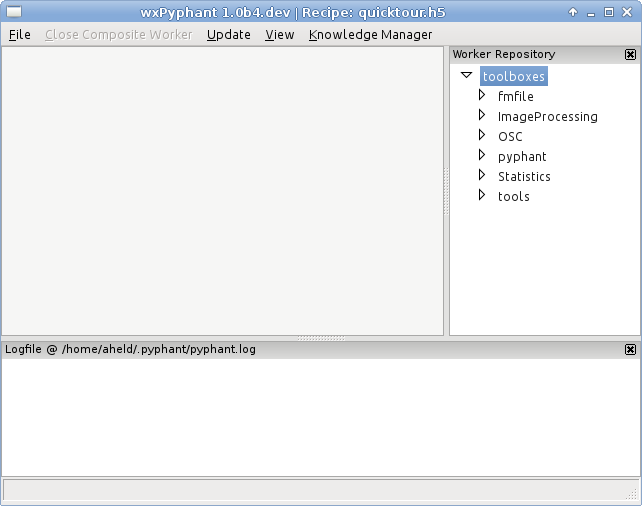
\includegraphics[scale=0.75]{fig/gui.png}
  \caption{Pyphant's graphical user interface}
  \label{fig:gui}
\end{figure}
The title bar shows pyphant's version and the recipe's filename. On
the right hand side, the installed toolboxes are listed in a tree
view. Each toolbox can be expanded to access the individual workers
contained in it. A worker can be placed on the central grey area
representing the recipe by a drag and drop operation. Let's try this
out with the |Load Image| worker from the |ImageProcessing|
toolbox. The drag and drop operation results in the worker appearing
on the central pane as depicted in \autoref{fig:gui_add_LI_worker}.
\begin{figure}[h]
  \centering
  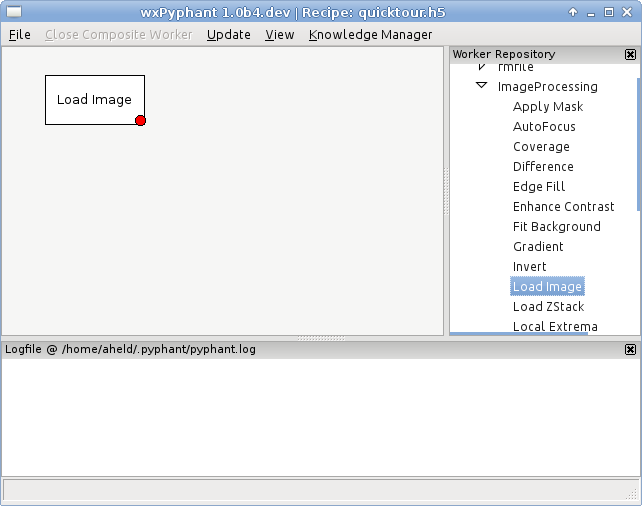
\includegraphics[scale=0.75]{fig/gui_add_LI_worker.png}
  \caption{Adding a worker to the recipe}
  \label{fig:gui_add_LI_worker}
\end{figure}
In order to be able to load an image, we have to tell pyphant about
its location. This is done by adjusting the |Filename| parameter of
the |Load Image| worker. For this purpose, simply click once onto the
worker. This brings up a dialog with all the adjustable parameters as
shown in \autoref{fig:gui_LI_worker_parameters}.
\begin{figure}[h]
  \centering
  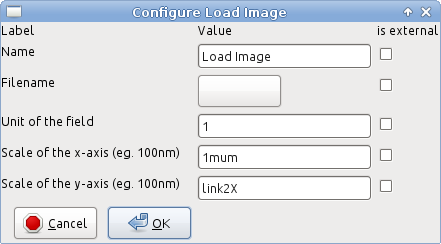
\includegraphics[scale=0.75]{fig/gui_LI_worker_parameters.png}
  \caption{Editing the parameters of a worker}
  \label{fig:gui_LI_worker_parameters}
\end{figure}
Clicking on the button to the right of the |Filename| label brings up
a file picker dialog. Use this dialog to select any image at hand.

The |Load Image| worker takes image data from a file and converts it
to pyphant's internal format. If the image has multiple color
channels, it will be converted to a gray scale image first. In our
case, the resulting internal format is a two dimensional
|FieldContainer|. In general, a |FieldContainer| is a discretized
scalar valued field with a unit for the field values and as many axes
as there are dimensions. An axis is itself a one dimensional
|FieldContainer|. The recursion is eventually ended by a sentinel
value for the dimensions. For further details also refer to
\autoref{sec:data_model} and Reference~\cite{pyphant}. As a side note
for the readers familiar with numpy\cite{numpy}, a |FieldContainer| is
an extension of a numpy array adding units, axes and some more
features. This explains the occurance of the three other parameters in
\autoref{fig:gui_LI_worker_parameters}. The default values are to
convert the image to a dimensionless field with a size of
\SI{1}{\micro\metre\squared}. The syntax for entering units is the
same as in the Full-Metadata Format\cite{Riede2010651}. The special
value |link2X| indicates to use the same scaling for the y-axis as for
the x-axis. You may leave these additional parameters as they are for
now. Note that the |Load Image| worker is not yet aware of image meta
data (such as Exif) indicating pixel size. This has to be entered
manually. Once you are satisfied with the parameter settings, press
|OK|.

Now we are ready to visualize the resulting |FieldContainer|. Before
doing so, we should note that a worker communicates with other workers
or visualizers via connectors. The input connectors on a worker are
called |Sockets| and the output connectors are called |Plugs|. In our
example, the worker has no |Sockets|, as it loads data from an
external source and it offers a single |Plug| where the
|FieldContainer| is made available shown as a red circle in the bottom
right corner. Pyphant uses lazy evaluation. That means that the actual
work of loading the image into memory and converting it into the
internal format is done only if the result of the |Plug| is
requested. In general, as long as we do not change any parameters and
all inputs on all |Sockets| are still the same, a cached result will
be used once a calculation has been triggered. We can trigger the
import of the image by requesting a visualization of it. This is done
by clicking with the alternate mouse button on the |Plug| in order to
bring up the context menu as shown in \autoref{fig:gui_context_menu}.
\begin{figure}[h]
  \centering
  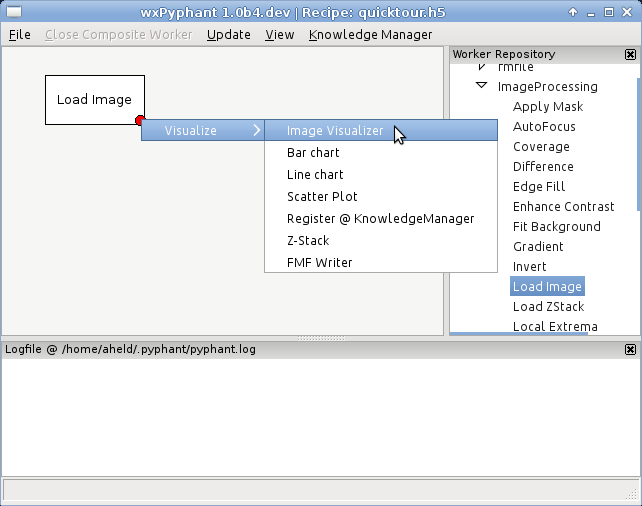
\includegraphics[scale=0.75]{fig/gui_context_menu.png}
  \caption{Visualizers are found by opening the context menu on a plug}
  \label{fig:gui_context_menu}
\end{figure}
The canonical choice for visualizing two dimensional |FieldContainers|
is the |Image Visualizer|. Selecting it will pop up a new window with
a false-color-visualization of the image data as in
\autoref{fig:gui_imagevis}.
\begin{figure}[h]
  \centering
  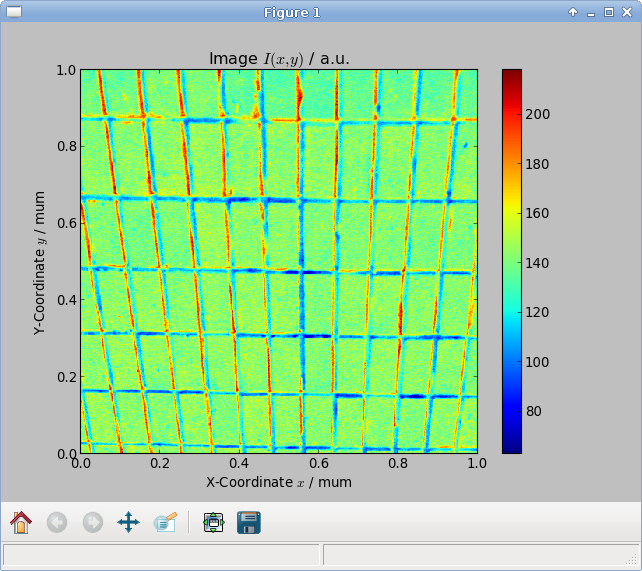
\includegraphics[scale=0.75]{fig/gui_imagevis.png}
  \caption{False-color visualization of a two dimensional FieldContainer}
  \label{fig:gui_imagevis}
\end{figure}
As some of the readers may have noticed, the |Image Visualizer| is
based on matplotlib\cite{matplotlib}. You may refer to matplotlib's
documentation on how to use the controls available in the toolbar of
the visualizer. As you can see in \autoref{fig:gui_imagevis}, the unit
of the field and the scalings of the axes are respected in the
visualization. If you want to choose another image, just go back and
edit the worker's |Filename| parameter until you are satisfied. We
have chosen a photography of a brick wall available for free
from~\url{http://sipi.usc.edu/database/}.

In a next step, we want to calculate the gradient magnitude of the
image we just imported. Pyphant already offers a worker for this
called |Gradient| also available in the |ImageProcessing|
toolbox. Please drag a |Gradient| worker into the recipe pane. As you
may have noticed, the |Gradient| worker not only offers a |Plug| in
the bottom right corner but also a |Socket| in the top left corner
indicated by a red square. In order to route the output from the |Load Image|
|Plug| to the |Socket| of the |Gradient| worker, simply connect
the two |Connectors| by a drag and drop operation starting on the |Plug|
and ending on the |Socket|. The link should be visible as an
arrow similar as in \autoref{fig:gui_gradient_worker}.
\begin{figure}[h]
  \centering
  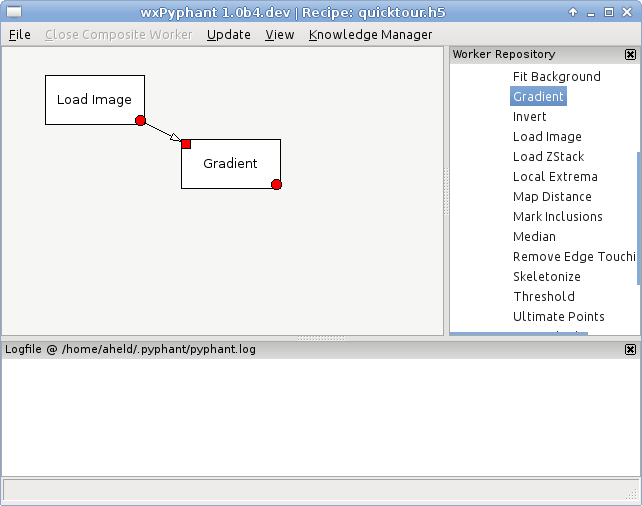
\includegraphics[scale=0.75]{fig/gui_gradient_worker.png}
  \caption{Information flow between workers is indicated by an
  arrow connecting the sockets}
  \label{fig:gui_gradient_worker}
\end{figure}
You may convince yourself that the |Gradient| worker offers no
parameters except for the possibility to rename it, which is always
available. As you have learned how to visualizing two dimensional
|FieldContainers| by now, you should be able to also visualize the
gradient magnitude. In \autoref{fig:gui_imagevis_gradient} we have shown
the visualizations of the original image and the gradient magnitude
side by side.
\begin{figure}[h]
  \centering
  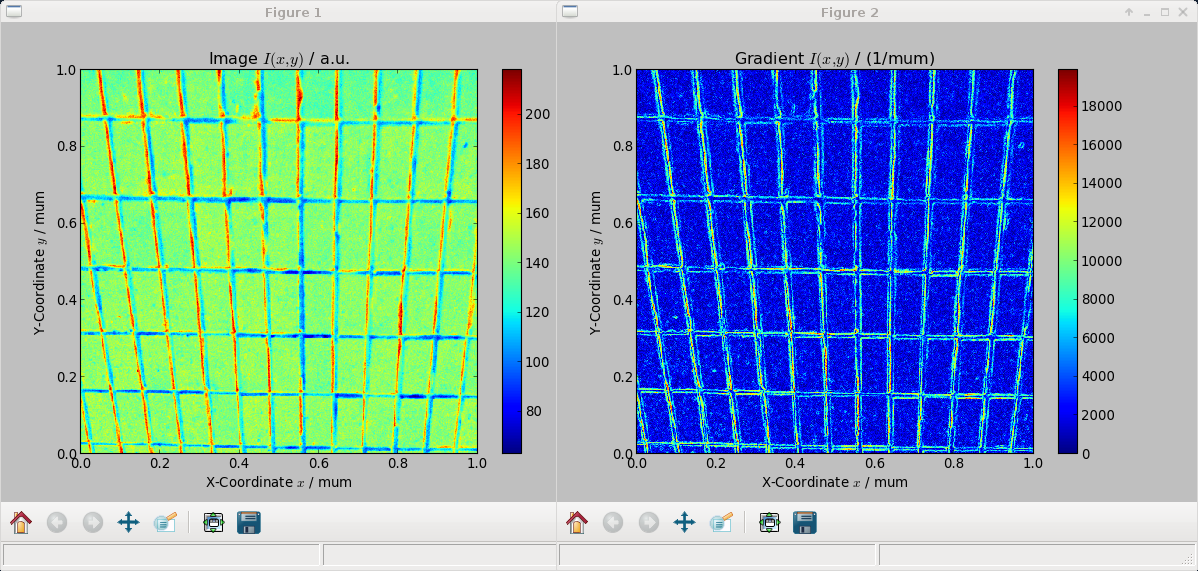
\includegraphics[width=\linewidth]{fig/gui_imagevis_gradient.png}
  \caption{Visualization of the original image (left) and its gradient
    magnitude (right)}
  \label{fig:gui_imagevis_gradient}
\end{figure}
Feel free to try the same on your recipe. Also note the correct
inference of the field unit of the gradient magnitude which is a first
order spatial derivative. The |Gradient| worker is unable to calculate
the gradient magnitude if the two axes of the original image are
incompatible. Try to set the axes units for instance to \si{m} and
\si{s}. You will get an error message and a python traceback will be
written to the log file which is also visible in the bottom of the
GUI. Go back and set both units to be compatible again.

In a last step, we add the |Histogram| worker from the |Statistics|
toolbox to the recipe. It takes a |FieldContainer| as input and
calculates a histogram of its field values as an output. In that case,
the output is a one dimensional |FieldContainer| irrespective of the
dimensionality of the input. You may want to set its |Bins| parameter
to a higher value than the default (10). Connect the |Gradient|
worker's output |Plug| to the |Socket| of the |Histogram| worker. Once
you're done with that, you can visualize the histogram by choosing the
|Bar chart| visualizer on the |Histogram| worker's |Plug| which is
appropriate for histograms. If you are uncertain about those steps, go
back and review how we connected the |Gradient| worker and visualized
its output. In our case, the resulting visualization for 50 bins is
shown in \autoref{fig:gui_barvis_histo} as a reference. Your result
may differ depending on the image you have chosen, its scaling and the
number of bins you entered.
\begin{figure}[h]
  \centering
  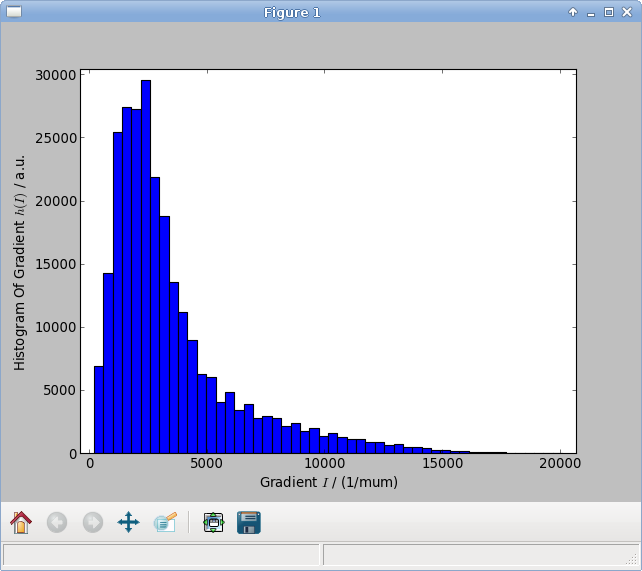
\includegraphics[scale=0.75]{fig/gui_barvis_histo.png}
  \caption{Bar chart visualization of a 50 bin histogram of the
    gradient magnitude}
  \label{fig:gui_barvis_histo}
\end{figure}

Having completed your first recipe, it is time to save it to
disk. The according menu items are found in the |File| menu. Also
notice the |Save results| checkbox in the |File| menu. It controls
whether the cached results of the workers should be saved to disk for
faster evaluation when reloading the recipe. You may uncheck it in
order to save disk space.

This completes the GUI part of the quick tour. In the next section, we
will learn how to write our own workers and visualizers and how to use
pyphant through its python API rather than through the GUI.

\FloatBarrier
\subsubsection{Extending and Scripting Pyphant}
\label{sec:introduction_extending_and_scripting}

For this part of the quick tour, we assume that the reader has a basic
knowledge of python\cite{python}, numpy\cite{numpy} and
scipy\cite{scipy}. If this is not the case, we recommend going through
some of the tutorials to be found on the respective homepages.

Let us begin by reformulating the above example by API calls instead
of graphical programming to get a first glimpse at pyphant's API. This
is shown in Listing~\ref{lst:api001}.

\begin{listing}[h]
  \inputminted[linenos]{python}{api001.py}
  \caption{The gradient magnitude histogram example in terms of API
    calls}
  \label{lst:api001}
\end{listing}

As can be seen from the import statements in lines 2 -- 5, the
toolboxes are separate python packages. Usually, a worker is located
inside its own module, but this is not necessarily the case. The core
of pyphant is found in the |pyphant.core| package. A recipe is also
known as a |CompositeWorker| and an empty one is created as shown in
line 8. Every parameter of a worker is an object. Paramters can be
accessed by the magic (i.e. auto-generated) attribute |param| followed
by the name of the parameter, where the first letter has to be
capitalized. The value of a parameter is accessed as shown in line 14.

|Sockets| and |Plugs| can be accessed by name, but since all the
workers in our little example have at most one |Socket| or |Plug|, it
is more convenient to pick them as the only entry in the list of all
|Sockets| or |Plugs| as shown in line 20, which also illustrates how
to connect a |Plug| and a |Socket|. The result of a plug is obtained
by calling |getResult| on it. The underlying numpy array of a
|FieldContainer| is accessed as its |data| member. We have skipped the
visualization of the |FieldContainers| in Listing~\ref{lst:api001} as
we will come back to visualizers in a minute.

IO in the HDF5 format is handled by the
|pyphant.core.H5FileHandler.H5FileHandler| class. Saving and loading a
recipe is shown in Listing~\ref{lst:api002}.

\begin{listing}[h]
  \inputminted[linenos]{python}{api002.py}
  \caption{Saving and loading a recipe}
  \label{lst:api002}
\end{listing}

The |H5FileHandler| is used as a context manager similar to python's
builtin |open|. It supports the file modes |'r'|, |'w'| and |'a'|
which stand for read, (over)write and append respectively.

When loading a recipe, you may wonder how to access the workers
contained in it. For this purpose, every worker has a unique name,
which happens to also be a parameter called
|Name|. Listing~\ref{lst:api003} shows how to access the |Gradient|
worker from the GUI example.

\begin{listing}[h]
  \inputminted[linenos]{python}{api003.py}
  \caption{Access a worker by name}
  \label{lst:api003}
\end{listing}


\section{Data Model}
\label{sec:data_model}

\subsection{Quantities}
\label{sec:data_model_quantities}

\subsection{Field Containers}
\label{sec:data_model_fcs}

\subsection{Sample Containers}
\label{sec:data_model_scs}

\subsection{Knowledge Manager}
\label{sec:data_model_knowledge_manager}

\section{Data Processing}
\label{sec:data_processing}

\subsection{Workers}
\label{sec:data_processing_workers}

\subsection{Recipes}
\label{sec:data_processing_recipes}

\subsection{Visualizers}
\label{sec:data_processing_visualizers}

\bibliographystyle{ieeetr}
\bibliography{bibliography}

\clearpage

\printindex

\end{document}

%%% Local Variables:
%%% TeX-PDF-mode: t
%%% End:
